\documentclass[a4paper, 12pt]{article}
\usepackage[total={17cm,25cm}, top=2.5cm, left=2.5cm, right=2.5cm,  includefoot]{geometry}
\usepackage[utf8]{inputenc}
\usepackage{array}
\usepackage{multirow}
\usepackage{hhline}
\usepackage{gensymb}
\usepackage{graphicx}
\graphicspath{ {} }
\usepackage[czech]{babel}
\usepackage{enumitem}
\usepackage{pdfpages}
\usepackage{amsmath}
\usepackage{verbatim}
\usepackage{listings}
\usepackage{hyperref}
\usepackage{amssymb}


\pagestyle{empty} % vypne číslování stránek




\usepackage[OT2,OT1]{fontenc}
\newcommand\cyr
{
\renewcommand\rmdefault{wncyr}
\renewcommand\sfdefault{wncyss}
\renewcommand\encodingdefault{OT2}
\normalfont
\selectfont
}
\DeclareTextFontCommand{\textcyr}{\cyr}
\def\cprime{\char"7E }
\def\cdprime{\char"7F }
\def\eoborotnoye{\char’013}
\def\Eoborotnoye{\char’003}


\begin{document}



\begin{titlepage}
\begin{center}
\noindent
\Large \textbf{České vysoké učení technické v Praze }\\ Fakulta stavební
\vspace{5cm}

\huge

%vložení loga cvut
\begin{figure}[h!]
	\centering
	
\includegraphics[width=7cm]{logo.png}
\end{figure}

\vspace{0.5cm}

Algoritmy v digitální kartografii \\

\vspace{3cm}

\Huge  
Geometrické vyhledávání bodu\\

\vspace{2cm}

\Large
Bc. Petra Pasovská \\
Bc. David Zahradník \\

\end{center}

\end{titlepage}




\pagestyle{plain}     % zapne obyčejné číslování
\setcounter{page}{1}  % nastaví čítač stránek znovu od jedné

\tableofcontents
\newpage

\section{Zadání}
\begin{figure}[h!]
	\centering
	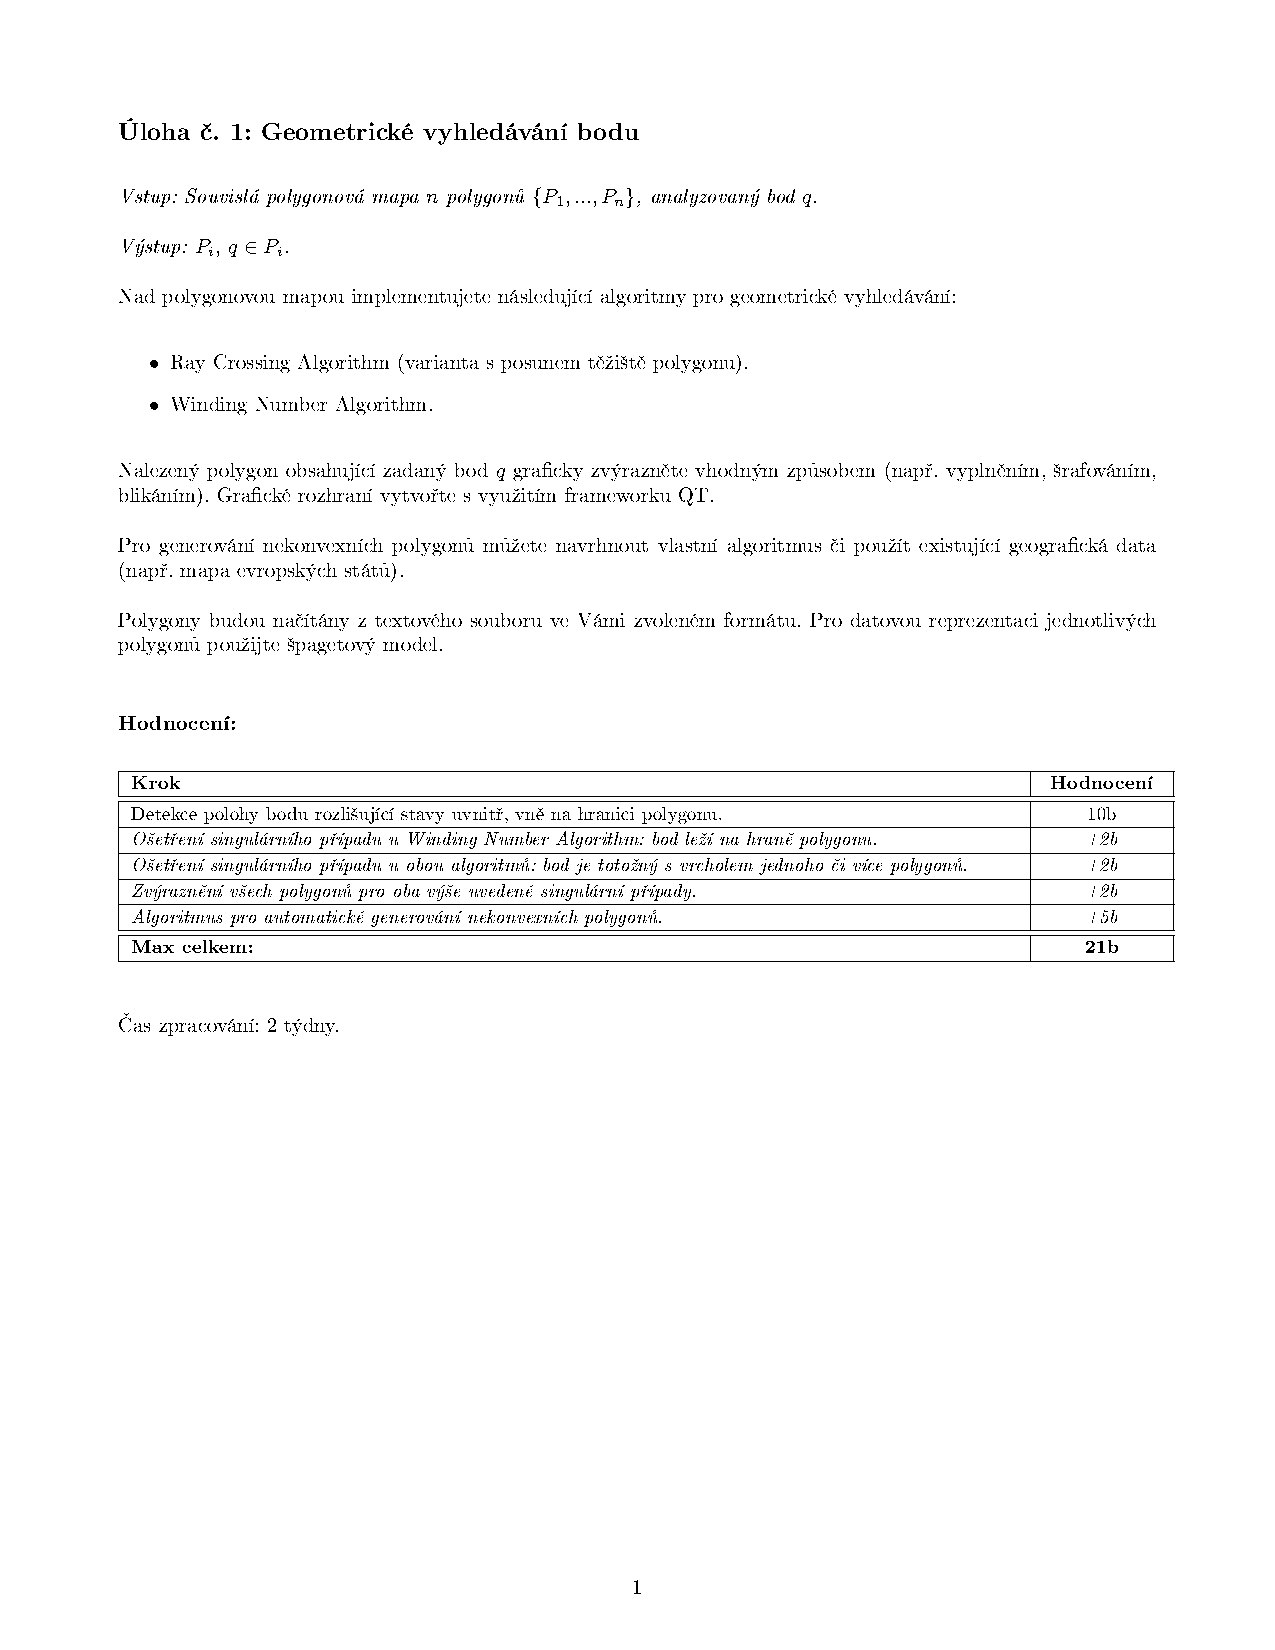
\includegraphics[clip, trim=0cm 10cm 0cm 3cm, width=1.2\textwidth]{zadani.pdf}
\end{figure}

\subsection{Údaje o bonusových úlohách}
V úloze byly vypracovány bonusové části týkající se ošetření singulárního případu u Winding Number Algorithm, kdy bod leží na hraně polygonu. Dále byl ošetřen singulární případ u obou algoritmů, kdy bod leží ve vrcholu jednoho či více polygonů. Pro oba výše zmíněné singulární případy byly zvýrazněny polygony. \\

?? Nekonvexní polygon? když se povede???


\clearpage

\section{Popis a rozbor problému}
Použít na důležité pojmy a objekty kurzívu/tučně, odřádkování apod ať to nějak vypadá!!!\\

Hlavním cílem této úlohy je tvorba aplikace, která uživateli určí pozici zvoleného bodu q. Termínem pozice je myšlen polygon, kterému zadaný bod přísluší.
\\

V závislosti na tvaru polygonu rozlišujeme dva základní typy. Jedná se o konvexní a nekonvexní polygon. Polygon můžeme označit za konvexní právě tehdy, pokud jsou všechny vnitřní úhly konvexní, tedy v případě, že úhly jsou menší nebo rovny hodnotě 180 $^\circ$. Zároveň pro takový polygon platí, že všechny přímky, jejichž oba krajní body leží uvnitř polygonu, mají s tímto polygonem všechny body společné. Takový polygon, který není konvexní, lze označit jako nekonvexní či konkávní.
\\

Porovnání konvexního a nekonvexního objektu lze vidět na následujícím obrázku.
\begin{figure}[h]
	\centering
	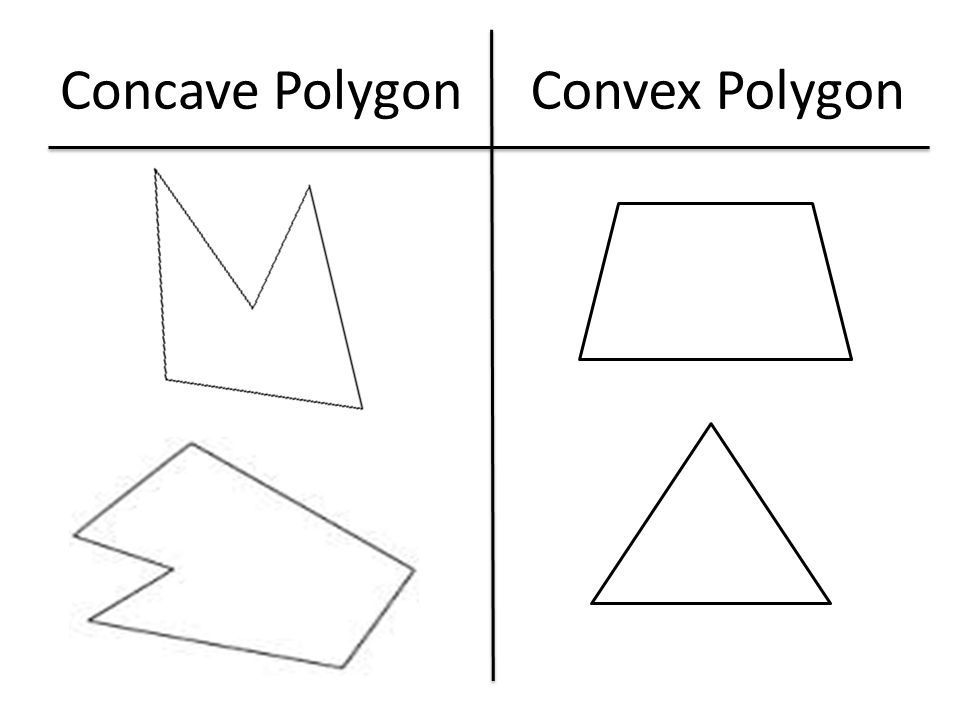
\includegraphics[width=10cm]{typy_polygonu.jpg}
	\caption{Porovnání konvexního a konkávního polygonu [zdroj: 1]}
\end{figure}

Bod q může mít vůči polygonu P jednu z těchto poloh:
\begin{enumerate}
\item Bod q leží uvnitř polygonu P.
\item Bod q leží vně polygonu P.
\item Bod q leží na hraně polygonu P.
\item Bod q je totožný s některým z vrcholu polygonu P.
\end{enumerate}


Pro určení pozice bodu q vůči polygonu existuje několik metod. V této aplikaci jsou implementován metody Ray Crossing Algorithm (varianta s posunem těžiště polygonu) a metoda Winding Number Algorithm.

\section{Popis použitých algoritmů}
Opět projet formu zápisu a vzhled!!!\\

Existuje mnoho metod pro určení pozice bodu q vůči polygonu P. Při volbě metod je vždy potřeba zhodnotit několik důležitých bodů, například požadavky vstupních/výstupních dat, časová náročnost či zda typ problému nespadá mezi NP problémy. V aplikaci byly použity algoritmy Ray Crossing Algorithm a Winding Number Algorithm. Mezi další známé metody pro určení pozice bodů patří třeba Line Sweep Algorithm (Zametací přímka), Divide and Conquer (Rozděl a panuj) či lze pozice určit i metodou hrubé síly (Brute Force Algorithm).

\subsection{Ray Crossing Algorithm}
Ray Crossing Algorithm lze do češtiny přeložit jako paprskový algoritmus. Primárně slouží k určení polohy bodu v konvexních mnohoúhelnících. Lze jej však zobecnit i pro nekonvexní. Obecně si lze metodu představit tak, že z libovolného bodu vedeme polopřímky a hodnotíme průsečíky přímky s hranami polygonu. \\

Označme si určovaný bod q. Z tohoto bodu je veden paprsek r (ray). Pokud si průsečík přímky r s hranami polygonu P označíme jako k, pak platí:
\begin{enumerate}
\item Pokud je k liché: Bod náleží polygonu P. $(q\in P)$ 
\item Pokud je k sudé: Bod nenáleží polygonu P.  $(q {\not \in} P)$ 
\end{enumerate}

\begin{figure}[h]
	\centering
	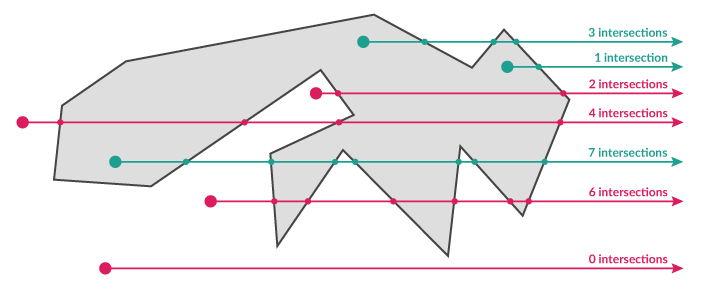
\includegraphics[width=10cm]{ray.png}
	\caption{Princip Ray Crossing Algorithm [zdroj: 2]}
\end{figure}

\subsubsection{Problematické situace}
Při použití Ray Crossing Algorithm může nastat několik problematických situací, které nelze opomenout. Tímto problémem jsou singularity. K singularitě v této metodě může dojít tehdy, pokud bod leží na hraně polygonu či pokud je bod totožný s některým z vrcholů polygonu. Z tohoto důvodu se využívá upravená varianta Ray Crossing Algorithm, kdy je provedena redukce souřadnic bodů 

\subsubsection{Implementace metody}
\begin{enumerate}
\item Nastavení počtu průsečíků rovno nule:  $ inters = 0 $ 
\item Redukce souřadnic x všech bodů polygonu vůči x-ové souřadnici bodu q:  $x'_i = x_i - x_q $ 
\item Redukce souřadnic y všech bodů polygonu vůči y-ové souřadnici bodu q:  $y'_i = y_i - y_q $ 
\item Volba podmínky:  $if(y'_i > 0)\&\&(y'_{i-1} <= 0)\|(y'_{i-1} > 0)\&\&(y'_{i} <= 0)  $ 
\item Při splnění podmínky:  $ x'_m = (x'_i y'_{i-1} - x'_{i-1} y'_i ) / (y'_i - y'_{i-1})$ 
\item Pokud $x'_m > 0$, zvýšení počtu průsečíků o jeden: $ inters = inters + 1 $
\item Určení zda počet průsečíků sudý či lichý: $if (inters\%2) = 0$, pak: $q\in P$ - počet průsečíků je sudý
\item V opačném případě: $q {\not \in} P$
\end{enumerate}

\subsection{Winding Number Algorithm}
Metoda ovíjení, či známá jako Winding Number Algorithm, je často používána pro určení pozice bodu vůči nekonvexnímu mnohoúhelníku. Algoritmus si lze představit tak, že se z určovaného bodu otáčíme postupně ke každému bodu polygonu a pokud se otáčíme po směru hodinových ručiček, úhel sčítáme, v opačném případě odčítáme. Pokud je výsledný úhel roven $2\pi$, lze říci, že bod náleží polygonu. V opačném případě nenáleží.

\begin{figure}[h]
	\centering
	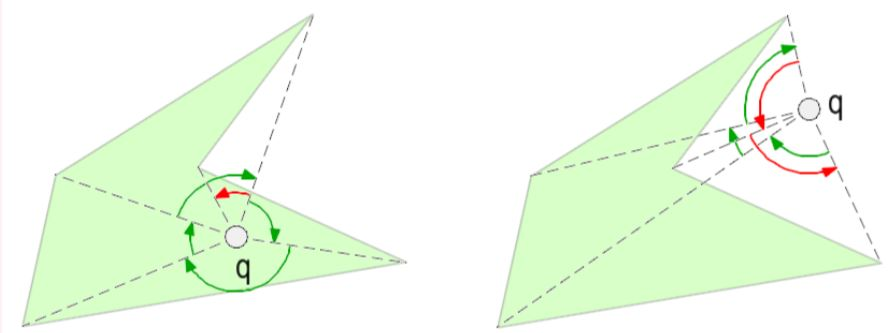
\includegraphics[width=10cm]{winding.jpg}
	\caption{Princip Winding Number Algorithm [zdroj: 3]}
\end{figure}

Při této metodě je zapotřebí si implementovat Winding Number $\Omega$. Pro $\Omega$ platí, že je rovna sumě všech rotací $\omega$ proti směru hodinových ručiček, které průvodič opíše nad všemi body: $ \Omega = \frac{1}{2\pi} \sum_{i=1}^n \omega_i^2$
\\
Orientace úhlů je dána:
\begin{enumerate}
\item Pokud je úhel $\sphericalangle p_i, q, p_{i+1}$ orientován ve směru hodinových ručiček, pak $\omega_i > 0$
\item Pokud je úhel $\sphericalangle p_i, q, p_{i+1}$ orientován proti směru hodinových ručiček, pak $\omega_i < 0$
\end{enumerate}


V závislosti na výsledné hodnotě $\Omega$ lze vyvodit následující závěry:
\begin{enumerate}
\item Pokud je $\Omega = 1$, pak platí $q \in P$ 
\item Pokud je $\Omega = 0$, pak platí $q { \not \in } P$
\end{enumerate}

\subsubsection{Problematické situace}
Pro Winding Number Algorithm je snadnější řešení singulárních případů. K těm dochází pouze v případě, že $q \approx p_i$.

\subsubsection{Implementace metody}
\begin{enumerate}
\item Nastavení výchozího úhlu $\omega$ rovno 0, volba tolerance $\epsilon$ : $\omega = 0, \epsilon = 1e-10$
\item Určení orientace $o_i$ bodu q ke straně $p_i, p_{i+1}$
\item Určení úhlu: $\omega_i = \sphericalangle p_i, q, p_{i+1}$
\item Volba podmínky - pokud pod vlevo: $\omega = \omega + \omega_i$
\item V opačném případě: $\omega = \omega - \omega_i$
\item Volba podmínky - pokud rozdíl: $(\omega - 2\pi) < \epsilon$, pak platí: $q \in P$
\item V opačném případě:  $ q { \not \in } P $
\end{enumerate}

\section{Vstupní data}
Mezi vstupní data patří analyzovaný bod q a textový soubor s body jednotlivých polygonů. Bod q je vkládán interaktivně po spuštění aplikace v grafickém okně. 
\\
\begin{itemize}
\item Analyzovaný bod q\\
Bod q je vkládán uživatelem interaktivně zmáčknutím levého tlačítka v grafickém okně aplikace.

\item Souvislá mapa polygonů\\
Vstupní soubor je ve formátu txt a obsahuje body jednotlivých polygonů.
\end{itemize}

Struktura vstupních dat:
[číslo bodu, souřadnice X, souřadnice Y]

Vstupní data musí být seřazená, tedy každý polygon v souboru musí začínat bodem jedna a končit n-tým bodem.  Ve vstupních datech je nový polygon dán číslem bodu jedna. Jednotlivé body se sekvenčně ukládají do proměnné QPointF a následně polygonu do QPolygonF. Všechny polygony se sloučí do proměnné  std::vector<QPolygonF>.

\section{Výstupní data}
Hlavním výstupem této úlohy je grafická aplikace, do níž je možné nahrát textový soubor s polygony a následně si body a mnohoúhelníky zobrazit. Zároveň je v aplikaci možné určit polohu bodu pomocí dvou metod. Dalším z výstupů jsou červeně zvýrazněné polygony v grafickém okně, které znázorňují polygon, kterému analyzovaný bod q náleží.
\\
+ pokud se podaří tvorba nekonvexních polygonů

\clearpage
\section{Aplikace}

\begin{figure}[h!]
	\centering
	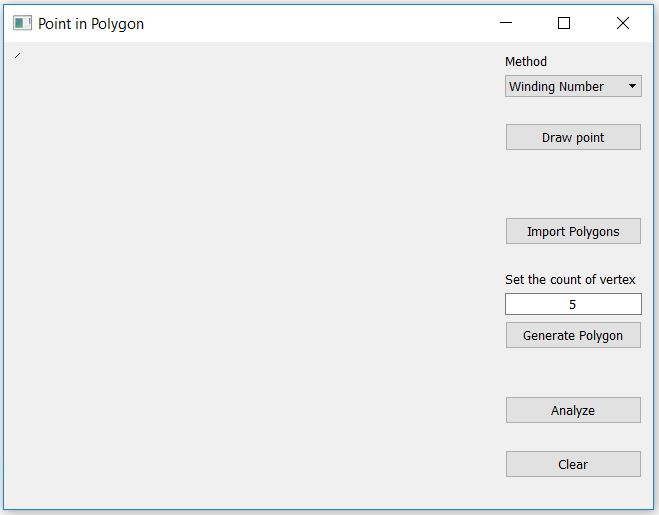
\includegraphics[width=10cm]{okno.jpg}
	\caption{Okno aplikace po spuštění kódu}
\end{figure}

\begin{figure}[h!]
	\centering
	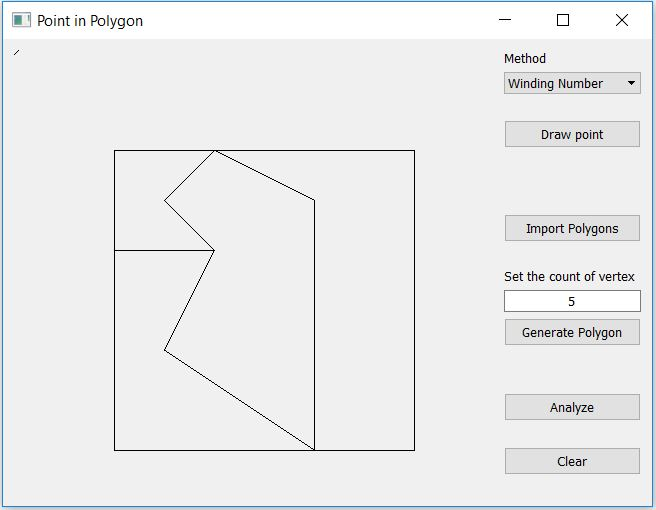
\includegraphics[width=10cm]{import.jpg}
	\caption{Naimportované souřadnice a jejich zobrazení v prostředí}
\end{figure}

\begin{figure}[h!]
	\centering
	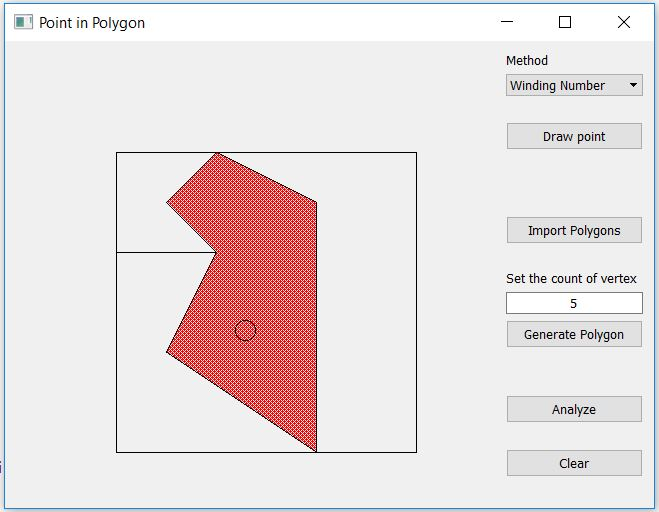
\includegraphics[width=10cm]{analyze_inside.jpg}
	\caption{Analýza polohy bodu za pomoci Winding Number Algorithm}
\end{figure}

\begin{figure}[h!]
	\centering
	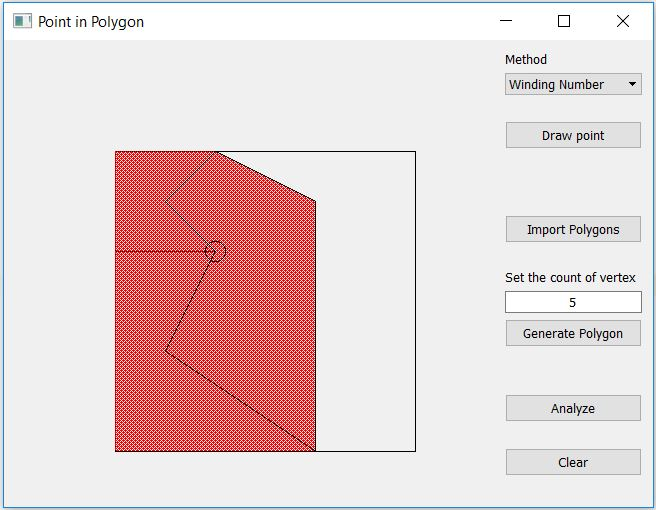
\includegraphics[width=10cm]{winding_vertex.jpg}
	\caption{Vyhodnocení Winding Number Algorithm při bodu totožném s vrcholem}
\end{figure}

\begin{figure}[h!]
	\centering
	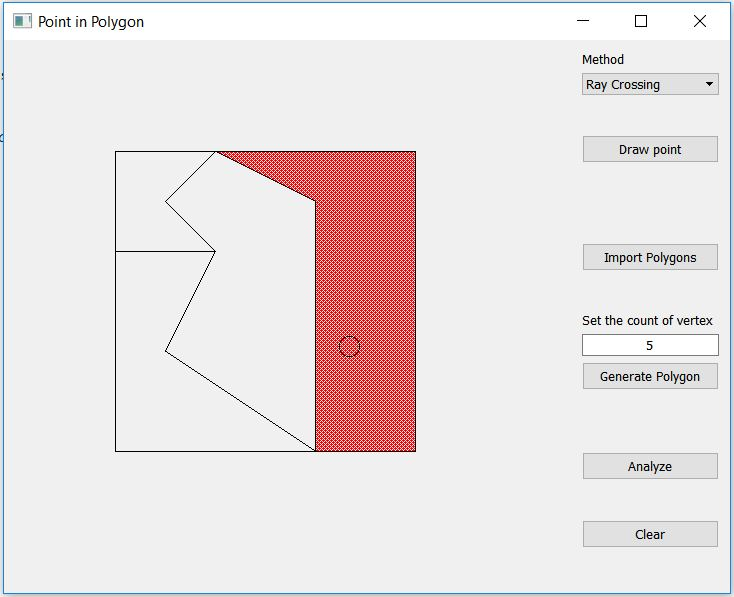
\includegraphics[width=10cm]{ray_inside.jpg}
	\caption{Analýza polohy bodu za pomoci Ray Crossing Algorithm}
\end{figure}

\begin{figure}[h!]
	\centering
	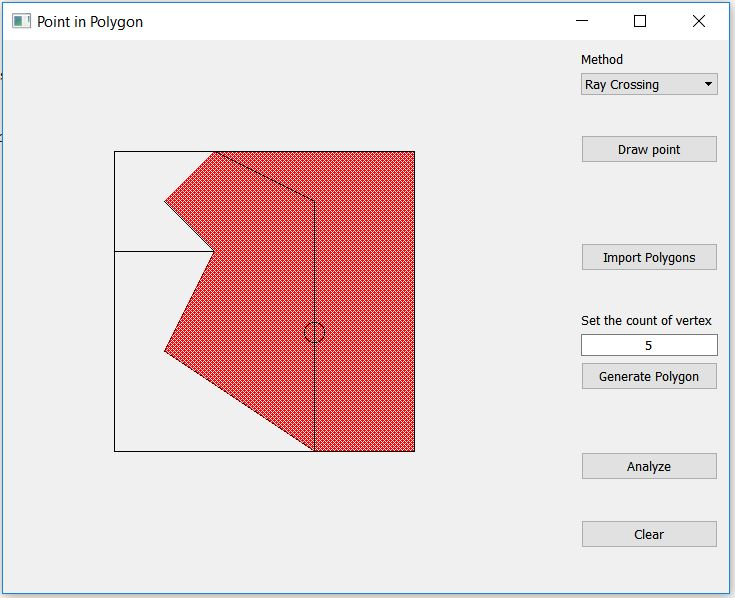
\includegraphics[width=10cm]{ray_boundary.jpg}
	\caption{Analýza polohy bodu na hraně za pomoci Ray Crossing Algorithm}
\end{figure}

\begin{figure}[h!]
	\centering
	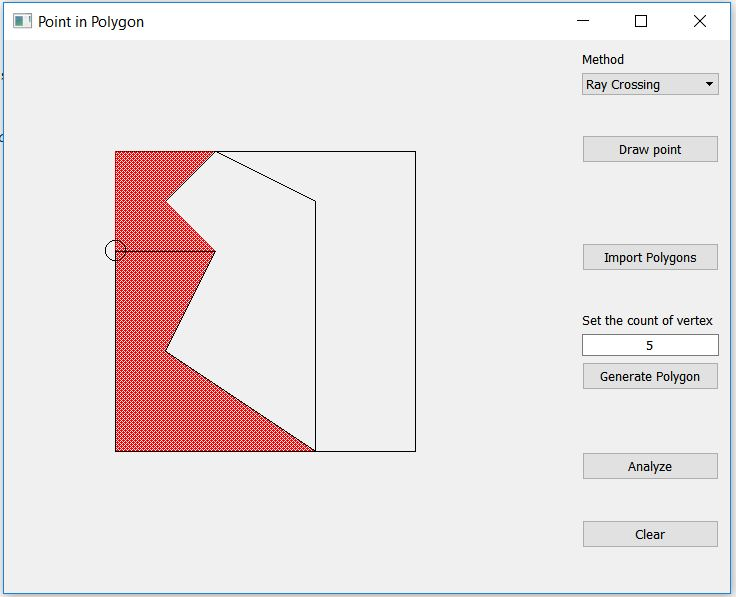
\includegraphics[width=10cm]{ray_vertex.jpg}
	\caption{Analýza polohy bodu ve vrcholu za pomoci Ray Crossing Algorithm}
\end{figure}

\begin{figure}[h!]
	\centering
	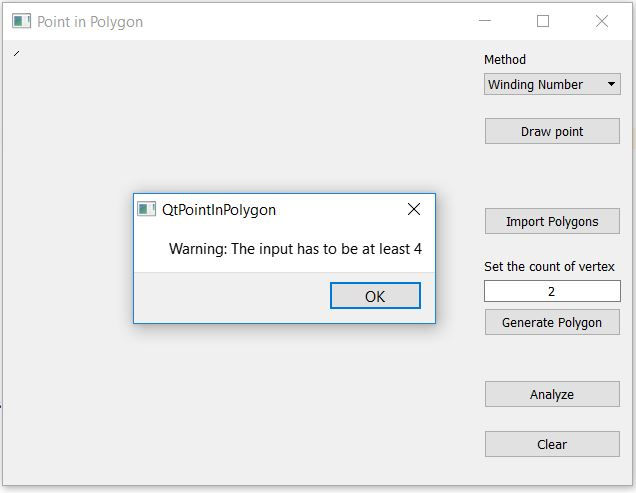
\includegraphics[width=10cm]{warning.jpg}
	\caption{Upozornění při vkládání nedefinované hodnoty}
\end{figure}

\clearpage

\section{Dokumentace}
\subsection{Třídy}
\subsubsection{Algorithms}
Třída Algorithms obsahuje celkem 6 metod. Metody jsou určeny pro výpočty použitých algoritmů.
\\

\textbf{getPositionRay}\\
Jedná se o funkci, která vypočítá geometrickou polohu bodu vůči polygonu za pomoci paprskového algoritmu (Ray Crossing Algorithm). Do funkce vstupuje určovaný bod \textit{q} a polygon, vůči kterému je poloha zjišťována. V případě, že výsledná hodnota funkce je rovna \textit{1}, znamená to, že bod leží v polygonu, případně na hraně či vrcholu polygonu. V ostatních případech leží bod mimo polygon.\\

\textbf{getPositionWinding}\\
Tato funkce určí polohu bodu vůči polygonu metodou ovíjení (Winding Number Algorithm). Vstupem je určovaný bod \textit{q} a polygon, vůči kterému je poloha určována. Výstupem může být některá z následujících hodnot. Pokud je výstupem celé číslo rovno \textit{1}, znamená to, že bod leží buďto ve vrcholu polygonu či na hraně polygonu. V případě, že výstupem je číslo \textit{0}, bod leží mimo polygon. Pokud nenastane žádná z uvedených možností, výstupem je hodnota \textit{-1}. Ve funkci je mimo jiné ošetřena singularita, která může nastat v případě, že bod leží ve vrcholu polygonu.\\

\textbf{getPointLinePosition}\\
Tato funkce má za úkol určit pozici bodu vůči linii. Do funkce vstupuje určovaný bod \textit{q} a dva body přímky, ve funkci značené \textit{a} a \textit{b}. Ze znalosti dvou bodů přímky jsme schopni určit determinant, jehož hodnotu následně porovnáváme se zvolenou minimální hodnotou, v tomto kódu označenou jako \textit{eps}. Pokud je hodnota determinantu větší než \textit{eps}, funkce vrací hodnotu \textit{1} a znamená to, že bod leží v levé polorovině. Pokud je hodnota determinantu menší než \textit{eps}, funkce vrací hodnotu \textit{0} a znamená to, že bod leží v pravé polorovině. Pokud nenastane ani jeden z výše uvedených závěrů, znamená to, že bod leží na hraně a výstupem je hodnota \textit{-1}.\\

\textbf{get2LinesAngle}\\
V této funkci je počítán úhel mezi dvěma hranami. Vstupem jsou 4 body typu QPointF. Nejprve je vypočten skalární součin vektorů a velikost obou vektorů. Úhel je poté vypočten jako arcus cosinus poměru skalárního součinu a součinu obou velikostí. Defaultně se v prostředí počítá v radiánech, je tedy zapotřebí na toto brát ohled, z toho důvodu máme veškeré vypočtené hodnoty úhlů převáděny na stupně. \\


\subsubsection{Draw}
Třída Draw obsahuje v private části několik objektů (

\subsubsection{Widget}

\subsection{Popis bonusových úloh}
\subsubsection{Ošetření singulárního případu u Winding Number Algorithm, kdy bod leží na hraně polygonu}
Uvnitř funkce je porovnávána velikost úhlu $\phi$. V případě, že rozdíl hodnoty $\phi$ a přímého úhlu je menší než zvolená mez (\textit{eps}), znamená to, že bod leží na hranici a návratová hodnota je rovna  \textit{1}.

\subsubsection{Ošetření singulárního případu u obou metod, kdy je bod totožný s vrcholem dvou a více polygonů}
Ve funkci getPositionWinding je na začátku kódu ošetřeno, zda vyhledávaný bod \textit{q} není totožný s některým z vrcholů. V případě, že ano, návratová hodnota je \textit{-1} a úhel ani umístění bodu vůči linii není počítáno. Následně je volena podmínka, pokud je návratová hodnota rovna \textit{-1}, funkce vrací číslo \textit{1} a bod se nachází ve vrcholu některých z polygonů. Ve funkci getPositionRay je využita hotová funkce pro určení pozice bodu vůči linii getPointLinePosition.

\subsubsection{Zvýraznění všech polygonů pro oba výše uvedené singulární případy}
Pokud je v kódu vyhodnoceno, že bod leží v některém z polygonů, návratová hodnota je rovna \textit{1}. Stejnou návratovou hodnotu mají i případy, kdy bod leží na hraně či ve vrcholu. Stačilo tedy jen napsat for-cyklus, který ověří všechny polygony a zvýrazní ty, pro něž je návratová hodnota rovna \textit{1}. 

\subsubsection{Tvorba nekonvexního polygonu}
Pro tvorbu polygonu je nutné zvolit počet vrcholů. Defaultně je hodnota nastavena na číslo 5. Ve funkci pro generování polygonů je na začátku uvedena podmínka, že vkládané číslo nesmí být menší než 4, neboť pokud bychom vložili tři body, vznikne trojúhelník a trojúhelník je vždy konvexní. V případě, že uživatel zadá číslo 3 nebo třeba text, zobrazí se okno, které upozorňuje na neplatný vstup. Při generování souřadnic byla původně použita knihovna RandomGenerator, ovšem tato knihovna je podporována pouze vyššími verzemi prostředí. Z toho důvodu je použita existující funkce rand a modulo 500, abychom byli schopni určitým způsobem regulovat oblast, ve které se bod zobrazí.

\clearpage
\section{Závěr}
Autoři splnili povinné zadání a některé bonusové úkoly. Vyhotovený program načte soubor polygonů a podle umístění značky stisknutím tlačítka myši spočítá, zda značka leží v polygonu či nikoli. \\

Ve funkci getPositionWinding jsou porovnány různé výsledky. Pokud není splněna při porovnání úhlu žádná z podmínek, návratová hodnota je rovna -1 a tato část je nadepsána komentářem "something else". Po zamyšlení, kdy by taková situace mohla nastat, nás napadla akorát taková možnost, kdy si definujeme prostor, ve kterém se polygony vykreslují a analyzovaný bod \textit{q} je umístěn mimo tento prostor (Out of range). V praxi by se mohlo jednat o takový případ, kdy budeme mít na vstupu zeměpisnou mapu Evropy a bod \textit{q} by vyjadřoval místo, které chceme navštívit a zvýrazněný polygon by znázornil danou zemi. V případě, že bychom zvolili místo v oceánu, nebyla by funkce pro tuto oblast definována a výstupem by byla hodnota -1. (LZE TO TAKTO NAPSAT? NEJSEM SI JISTÁ JESTLI TO ÚPLNĚ DOBŘE CHÁPU, ALE U KOMENTÁŘE JSOU OTAZNÍKY, TAK ASI NENÍ ÚPLNĚ ŠPATNÝ SE NAD TÍM ZAMYSLET :-)


\subsection{Náměty na vylepšení}
\subsubsection{Zobrazení dat}
Jelikož program má předdefinovanou velikost vykreslovacího okna, načtená data mimo toho okno se nezobrazí. Tento problém by se dal řešit transformací velikosti okna.

\subsubsection{Souřadný systém}
Vykreslovací okno vývojového prostředí Qt má souřadný systém s definovaný počátkem v levém horním rohu,  kladnou osou X vpravo a kladnou osou Y vzhůru. Souřadný systém v Qt se liší od používaných souřadných systémů (matematických i kartografických), proto se importovaná data nezobrazí, jak by uživatel očekával. Řešením by byla transformace bodů.

\subsubsection{Určovaný bod q}
Při určování pozice bodu \textit{q} se vždy řeší jeho pozice ve středu. Při testování jednotlivých funkcí a podmínek bylo poměrně náročně trefit vrchol či hranu. Vhodné by bylo, aby byla porovnávána i pozice bodů ležících no hlavních poloosách. Nejideálnější řešení by bylo, pokud bychom byli schopni porovnávat celkovou plochu, kterou bod zaujímá, i pro uživatele by to bylo jednodušší pro představu. Přesto by zde mohl být v některých případech problém s nižší přesností.

\subsubsection{Datový typ funkcí ve třídě Algorithm}
Při vyhodnocování jednotlivých funkcí je pro nás podstatné, zda je návratová hodnota rovna jedné. Ostatní případy nás nezajímají. Po zamyšlení by zřejmě bylo vhodné, pokud bychom datový typ zvolili bool místo int. Přesto pokud bychom chtěli brát v úvahu i rozšířené situace, kdy by se bod dostal mimo dosah, je vhodnější použít datový typ int a v případě, že by tak nastalo, přes funkci QMessageBox zobrazit zprávu, že bod se nachází Out of Range. 


\clearpage
\section{Reference}

\begin{enumerate}
\item  Presentation about convex and concave polygons [online][cit. 21.10.2018]. \\
Dostupné z: https://slideplayer.com/slide/6161031/  \\
\item  Introducing Wherewolf - A serverless boundary service from WNYC [online][cit. 21.10.2018]. \\
Dostupné z: https://source.opennews.org/articles/introducing-wherewolf/  \\
\item  BAYER, Tomáš. Geometrické vyhledávání [online][cit. 21.10.2018]. \\
Dostupné z: https://web.natur.cuni.cz/~bayertom/images/courses/Adk/adk3.pdf  \\

\end{enumerate}
\end{document}



 